\chapter{Testing in Scratch}

\section{Background and Related Work}

\begin{wrapfigure}{r}{0.5\textwidth}
    \centering
    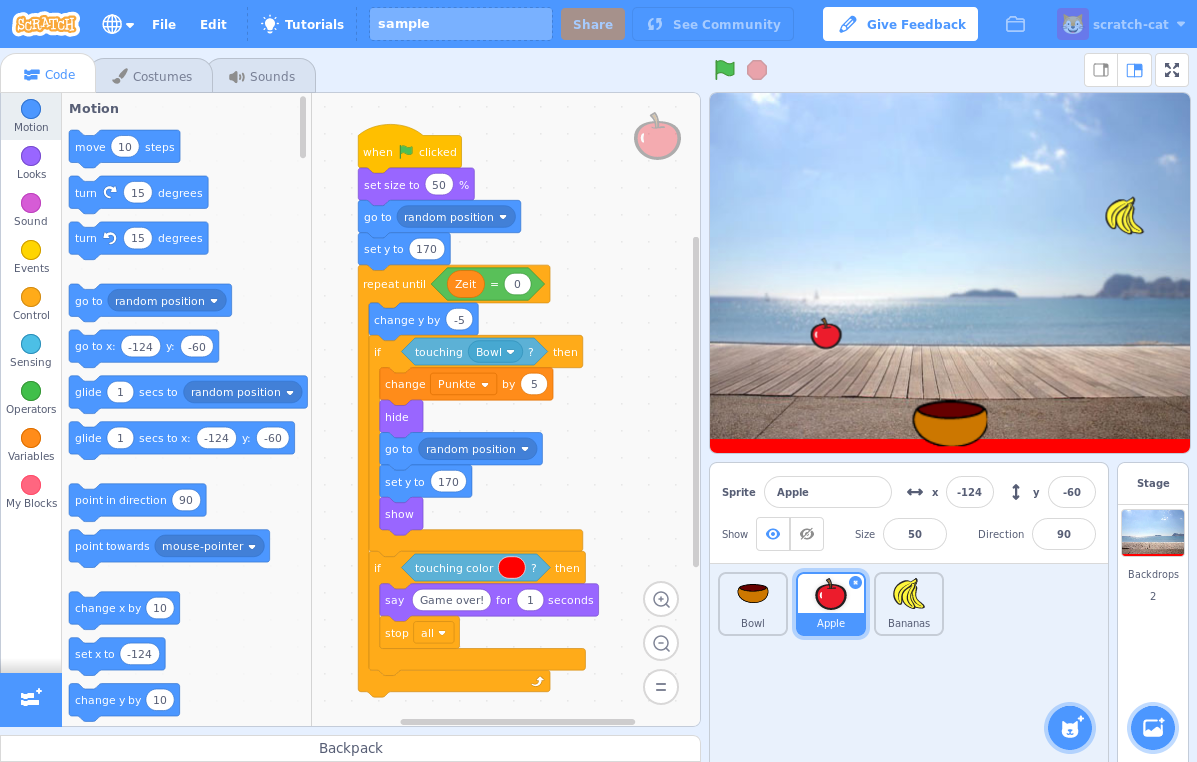
\includegraphics[width=0.4\textwidth]{scratch-example}
    \caption{The Scratch Interface}
    \label{fig:the_scratch_interface}
\end{wrapfigure}
=== Scratch
- block based programming language currently developed by the MIT Media Lab \cite{scratch}
- code controls sprites on a two-dimensional stage according to user input from mouse keyboard or other sources (extensions)
- creates a interactive animated project
- Graphics and audio can easily be integrated into Scratch projects
- attractive for teaching beginner courses on programming because ...
    - block based code eliminates syntax errors and makes it intuitive
    - integrating media into the project facilitates creativity (and is more fun for younger students)

- However, the multimedia nature of Scratch programs also makes automated assessment difficult
$\rightarrow$ automatic assessment of Scratch programs is still an open problem
- At least two other projects have tackled the task of automatically assessing Scratch projects.

=== Hairball
- Hairball \cite{hairball} allows static analysis of scratch programs
- Written in python
- Takes the source file of a scratch project and performs static analysis
- Has a plugin-based architecture
    - Comes with pre-defined plugins
    - allows to define own plugins, which iterate over the scratch blocks to analyze them
- Possible use cases:
    - check if students use a new construct, which the exercise focuses on
    - detect code smells
    - measure the complexity of a program $\rightarrow$ see Dr.Scratch
- Since it only allows static analysis, not suitable to check the functionality of a program

=== ITCH
- ITCH (Individual Testing of Computer Homework for Scratch Assignments) \cite{itch}
- Replaces constructs in the Scratch project
    -> allows simple textual input-output testing with pre-defined values using "ask" and "say" blocks
    - "ask" and "say" blocks are used in Scratch to ask the user for textual input and to display textual output on the screen
      (use cartoon speech bubbles)
- This, however,  only allows to test projects with a small subset of Scratch functionality
- Not very useful in general for Scratch because it focuses on multimedia and creativity
- Other languages (also block languages [citation needed]) are better suited for this task

\section{Caveats}
- Runtime testing of Scratch programs has some caveats
- This section explains some critical details that make testing of Scratch programs difficult

=== Parallel scripts
- Individual testing of program parts problematic
    - Scratch runs multiple scripts in parallel
        - Scripts often depend on one another
    - Not very useful to test single program parts
    - Possible to define multiple independent scripts that each activate with a different button press
        - but becomes convoluted
        - but defeats to purpose of Scratch to create a interactive environment
$\rightarrow$ Use a complete black box approach
    - Scratch programs are controlled by simulating user input instead of manually calling certain scripts
    - The only information, which is checked, is what appears on screen
        - properties of sprites and variables

=== Lack of IO, multimedia nature
- Scratch has a Lack of traditional IO mechanisms
    - makes it hard to extract information about the current program state
    - makes it hard to control the execution of a Scratch program
    - no traditional input output testing possible without limiting the project to a small subset of Scratch's functionality
$\rightarrow$ Give test cases an interface that can be used to interact with the Scratch project
    - interacts directly with the Scratch virtual machine
    - a way to get information about sprites and variables
    - a way to simulate user input

=== Scratch programs depend on real time
- Scratch blocks that involve timings, like "wait" or "say for secs" use real time to delay execution
$\rightarrow$ Scratch programs can not be sped up for testing
$\rightarrow$ Since Scratch 3.0 runs in a single-threaded environment (JavaScript), running multiple instances
              at once will influence the execution

=== Many tested properties will depend on time
- A tested property might depend on a previous value
    - e.g. check if a sprite is moving right
    - sprites save the values from the previous execution step
- Some tested properties should hold for a time or for the whole execution
    - Provide a way to define constraints that must always hold

\section{Approach}
- Each test case executes the program exactly once
- During the test, user input is simulated to control the program
- Then, the resulting changes (movement, animation, etc.) are checked by the test through traditional assertions
- The test must be able to control the program execution
    - e.g. save some information about the sprite, run the program for a second, then compare

=== Shortcomings of this approach
- Scratch projects need to be well defined to be tested
    - Can take the creativity out of the process, but can also give the students a guide to follow, which helps them to not get stuck on one problem
    - Students can test their programs with the test suite beforehand on their own to verify their programs
    - Problem: might incentivize students to try to cheat the tests
        $\rightarrow$ Automated testing should only be used in conjunction with static analysis, manual analysis, or random secret tests
        (static analysis should easily show anomalies on the projects)

=== Advantages
- Students can test their programs with the test suite beforehand on their own to verify their programs
    $\rightarrow$ Students can easily receive feedback and will change their programs according to the tests
    $\rightarrow$ Incentivizes students to ask for help if they can't progress, because the test clearly shows that there is a problem


